% Using KOMA Script document style
% Font size setting and
% option to skip empty lines as new paragraphs
\documentclass[10pt,a4paper]{article}
% Packages without Options
\usepackage{
	algorithm,
	alltt,
	algpseudocode,
	amsfonts,
	amssymb,
	appendix,
	array,
	booktabs,
	dirtree,
	enumitem,
	float,
	footnote,
	gensymb,
	geometry,
	graphicx,
	interval,
	karnaugh-map,
	lipsum,
	listings,
	longtable,
	makecell,
	mathtools,
	minted,
  nicematrix,
	parskip,
	pdfpages,
	pgfkeys,
	pgfplots,
	subcaption,
	tabularx,
	tablefootnote,
	textcomp,
	tikz,
    titlecaps,
	venndiagram,
	wrapfig,
	wrapfig,
	xcolor
}



% Packages with Options

\usepackage[framemethod=tikz]{mdframed}
\usepackage[colorlinks,linkcolor=cyan, citecolor=cyan, urlcolor=cyan]{hyperref}
\usepackage[labelfont=bf,textfont=it,labelsep=period]{caption}
\usepackage[RPvoltages]{circuitikz}
\usepackage[english]{babel}
\usepackage[nameinlink,noabbrev]{cleveref}

\definecolor{mintedbackground}{rgb}{0.97,0.97,0.97}

\setminted[cpp]{
bgcolor=mintedbackground,
    linenos=true,
    breaklines=true,}

\setminted[js]{
bgcolor=mintedbackground,
    linenos=true,
    breaklines=true,}

\setminted[python]{
bgcolor=mintedbackground,
    linenos=true,
    breaklines=true,}
    

\linespread{1.5}

% Package: AlgorithmicX
% Sets all comments to be indentend and aligned

\renewcommand{\Comment}[2][.7\linewidth]{%
  \leavevmode\hfill\makebox[#1][l]{//~#2}}


% Package: Interval
% Sets the style of mathematical intervals
\intervalconfig{
soft open fences, separator symbol=,,
}

% Package: Geometry
% Sets the page margins
\geometry{
    a4paper,
    left=32mm,
    right=22mm,
    top=22mm,
    }
	
% Creates a proper caption name for algorithms
\newcommand{\algorithmautorefname}{Algorithm}
\newcommand{\listingautorefname}{Listing}
\algrenewcommand{\algorithmiccomment}[1]{\texttt{// #1} }
% Creates a numbered environment for Theorems
\newtheorem{theorem}{Theorem}

% Redefine the implication arrow to be a simple, thin arrow instead of the default, thick arrow
\renewcommand{\implies}{\rightarrow}

% Create a new command for the set complement to make my logical statements easier to read
\newcommand{\compl}{\overline}

% Creates commands for combinatorics nCr and nPr
\newcommand{\nCr}[2]{\,_{#1}C_{#2}} % nCr
\newcommand{\nPr}[2]{\,_{#1}P_{#2}} % nPr

% Package: tikz
% Loads libraries for drawing automata, 
\usetikzlibrary{automata,positioning,shadows,arrows, shapes.gates.logic.US, calc}

% Creates a command to create a button shape
\newcommand*\keystroke[1]{%
  \tikz[baseline= (key.base)]
    \node[%
      draw,
      fill=white,
      drop shadow={shadow xshift=0.25ex,shadow yshift=-0.25ex,fill=black,opacity=0.75},
      rectangle,
      rounded corners=2pt,
      inner sep=1pt,
      line width=0.5pt,
      font=\scriptsize\sffamily
    ] (key) {#1\strut};
}

% Package: pgfplot
% Sets the global options for PGF Plots
\pgfplotsset{compat=newest}

% Package: tikz
% Flowchart Shapes
\tikzstyle{startstop} = [rectangle, rounded corners, minimum width=3cm, minimum height=1cm,text centered, draw=black, fill=red!30]
\tikzstyle{io} = [trapezium, trapezium left angle=70, trapezium right angle=110, minimum width=3cm, minimum height=1cm, text centered, draw=black, fill=blue!30]
\tikzstyle{process} = [rectangle, minimum width=3cm, minimum height=1cm, text centered, draw=black, fill=orange!30]
\tikzstyle{decision} = [diamond, minimum width=3cm, minimum height=1cm, text centered, draw=black, fill=green!30]
\tikzstyle{arrow} = [thick,->,>=stealth]

% Disable Minted syntax error highlights (red boxes)
\AtBeginEnvironment{minted}{%
  \renewcommand{\fcolorbox}[4][]{#4}}

% Listings Style (non-minted)

\lstdefinestyle{arjuncode}{
    basicstyle=\ttfamily,
    breakatwhitespace=false,         
    breaklines=true,                 
    captionpos=b,                    
    keepspaces=true,                 
    numbers=left,                    
    numbersep=5pt,                  
    showspaces=false,                
    showstringspaces=false,
    showtabs=false,                  
    tabsize=2
}

\lstset{style=arjuncode}

\graphicspath{{images/}}


\title{CM2005: Object-Oriented Programming \\ End-of-Term Assignment}
\author{Arjun Muralidharan \\ University of London}
\begin{document}

\maketitle
\newpage
\tableofcontents
\listoffigures
\listoftables
% \listofalgorithms

\newpage
\renewcommand{\subsubsectionautorefname}{section\negthinspace}

\section{Introduction}
This report documents how the OtoDecks application was extended to fulfil the requirements for the end-of-term assignment. The application uses the starter code from Week 19 in the module.

\begin{figure}[H]
	\centering
	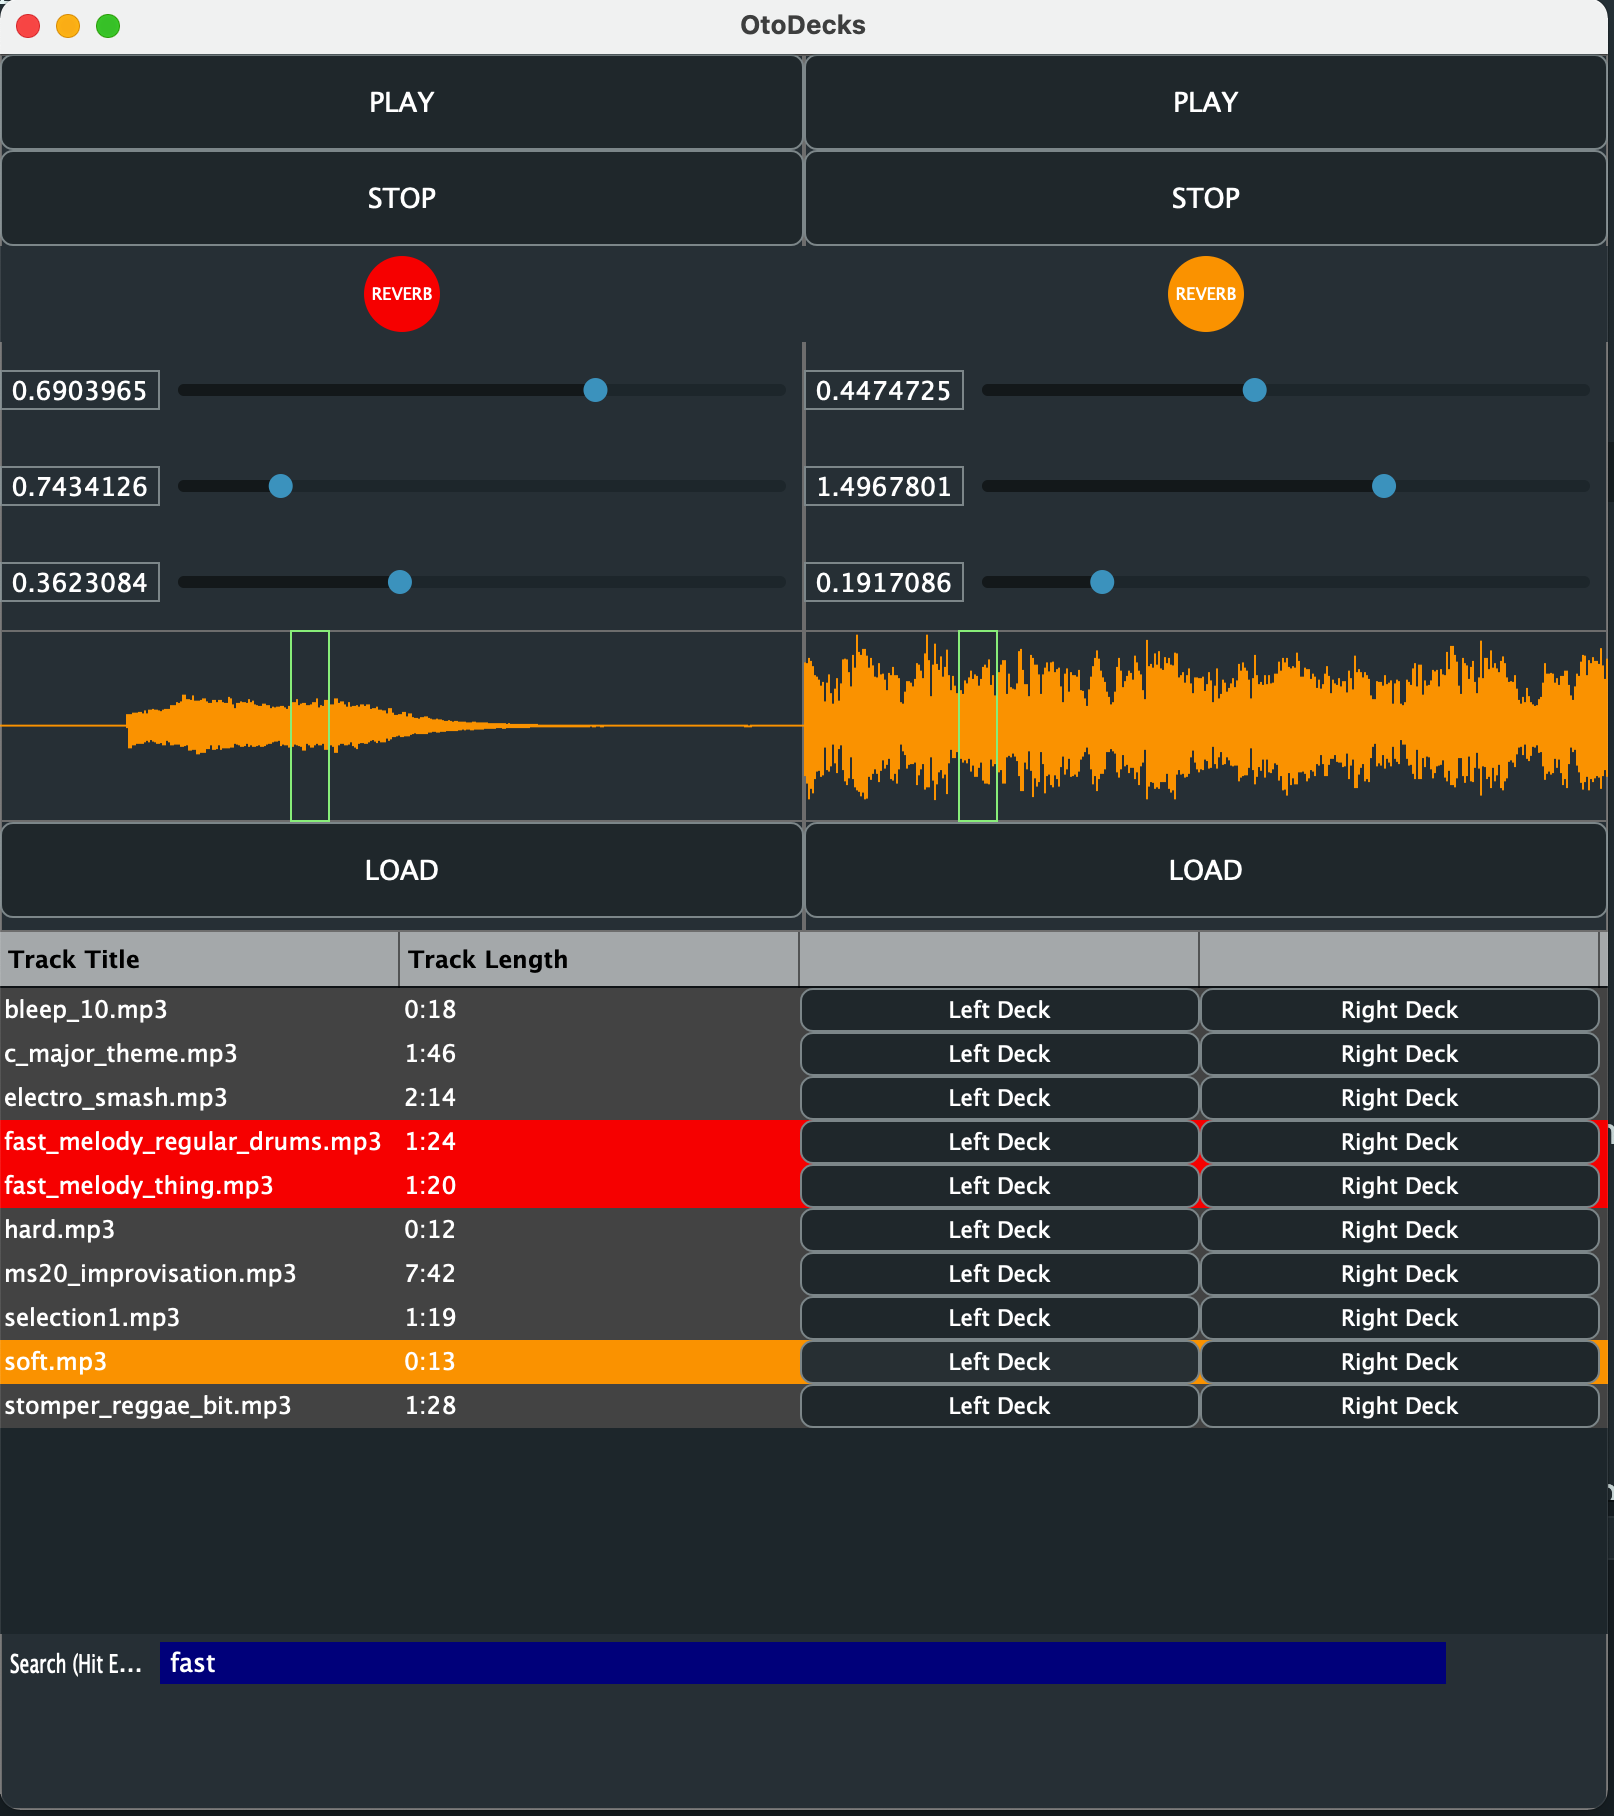
\includegraphics[width=13cm]{fullapp.png}
	\caption{Completed OtoDecks Application}
	\label{endlibrary}
\end{figure}

\section{R1: Custom Deck Control}
The custom deck control implemented in this application is a button to toggle a reverb effect. It uses a built-in JUCE reverb class. In order to fulfill the requirement of custom graphics, a separate custom JUCE component was create.
\subsection{R1A: Custom Graphics}
Custom graphics were achieved by creating a separate, custom \texttt{CustomDeckControl} class which has its own \texttt{paint()} function. As the class inherits from \texttt{TextButton}, the \texttt{paint()} function was replaced by a \texttt{paintButton()} function as recommended by the JUCE documentation. This allowed reacting to user interaction with the button.

The graphical aspect was achieved by drawing an ellipse with dedicated colour states for mouse hovering and mouse clicks. A toggle capability was implemented by introducing a public data member on the class, \texttt{toggle}, storing the state of the toggle as a boolean value. If the component is clicked, the toggle value is flipped. The actual toggling happens in the \texttt{DeckGUI} class, which has the listener for this custom component.

\begin{listing}[H]
	\begin{minted}{cpp}
// Toggle the reverb audio effect
if (button == &reverbButton)
{
	player->toggleReverb();
	reverbButton.toggle = !reverbButton.toggle;
}
	\end{minted}
	\caption{Toggling the graphical state in DeckGUI}
	\label{reverb}
\end{listing}

The final result is a toggle button that was placed right below the play and stop buttons.

\begin{figure}[H]
	\centering
	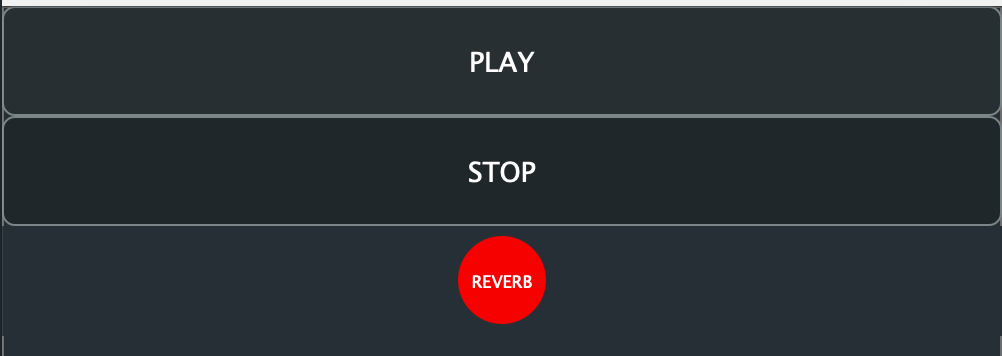
\includegraphics[width=9cm]{reverb.png}
	\caption{Custom Deck Control with Custom Graphics}
\end{figure}

\subsection{R1B: Playback Control}
To actually apply a reverb effect, the function \texttt{toggleReverb} in the \texttt{DJAudioPlayer} class was created. It is called as shown in \autoref{reverb} and the function itself toggles a private boolean data member in the \texttt{DJAudioPlayer} class. In order to handle the reverb, a separate \texttt{AudioTransportSource} was needed based on JUCE's \texttt{ReverbAudioSource} class. Based on the toggle, either this transport source will be used, or the regular \texttt{resampleSource}. This logic is implemented in the \texttt{getNextAudioBlock} function of the audio player as shown in \autoref{reverbsource}.

\begin{listing}[H]
	\begin{minted}{cpp}
void DJAudioPlayer::getNextAudioBlock(const AudioSourceChannelInfo& bufferToFill)
{
	// Switch to the reverb source if reverb is active
	if (reverb == true)
	{
		reverbSource.getNextAudioBlock(bufferToFill);
	}
	// Otherwise use the regular resample source
	else
	{
		resampleSource.getNextAudioBlock(bufferToFill);
	}
}
	\end{minted}
	\caption{Switching the audio source for reverb}
	\label{reverbsource}
\end{listing}

\section{R2: Music Library}
\subsection{R2A: Add Files}
Adding files to the music library has been implemented using file drag and drop capabilities in JUCE. All of this functionality was implemented in the \texttt{PlaylistComponent} class. All tracks are stored by file path in the \texttt{trackTitles} array, as shown in \autoref{addfiles}. The tracks are added using the \texttt{paintCell} function to the first columns of the table constructed in the constructor function of \texttt{PlaylistComponent}. 

\begin{listing}[H]
	\begin{minted}{cpp}
void PlaylistComponent::filesDropped(const StringArray &files, int x, int y)
{
	// Iterate over all dropped files and store the track titles and lengths into vectors
	for (String file : files)
	{
		trackTitles.push_back(file); 
	}

	// Refresh the table to show the newly added files
	tableComponent.updateContent();
}

/************************/

void PlaylistComponent::paintCell(Graphics &g,
					int rowNumber,
					int columnId,
					int width,
					int height,
					bool rowIsSelected)
{

	// Insert the track titles into the first column of the library
	if (columnId == 1)
	{
		g.drawText(File{trackTitles[rowNumber]}.getFileName(),
				   2, 0,
				   width - 4, height,
				   Justification::centredLeft,
				   true);
	}

}

	\end{minted}
	\caption{Adding files to the application}
	\label{addfiles}
\end{listing}

\subsection{R2B: Meta Data}
As shown in \autoref{addfiles}, only the track file names (without the full path) are shown to the user. We are parsing this information by running the path names through the \texttt{getFileName()} function. Additionally, we are calculating the time length of specific track in the \texttt{getLengthOfTrack} function that was custom implemented. This function receives a file name and returns the length as a string in "MM:SS" format. This procedure is shown in \autoref{getlength}.

\begin{listing}[H]
	\begin{minted}{cpp}
String PlaylistComponent::getLengthOfTrack(String file)
{
	auto duration{0};

	// Calculate the duration of the track by using an AudioFormatReader on the audio file
	std::unique_ptr<juce::AudioFormatReader> reader(formatManager.createReaderFor(File{file}));
	if (reader.get() != nullptr)
	{
		// Formula to calculate length based on sample size and sample rate
		duration = (float)reader->lengthInSamples / reader->sampleRate;
	}

	// Calculate minutes and seconds
	String minutes = std::to_string(duration / 60);
	String seconds = std::to_string(duration % 60);

	// If the track doesn't have any seconds beyond the full minute, we need to append another 0
	// Otherwise tracks that are e.g. 5 minutes long show up as "5:0" instead of "5:00".
	if (seconds == "0")
	{
		seconds = "00";
	}

	// Return the combined track length in MM:SS format
	return minutes + ":" + seconds;
}
	\end{minted}
	\caption{Calculating track lengths}
	\label{getlength}
\end{listing}

These track lengths are retrieved at the moment when files are dropped into the library and stored in a vector, similar to the track titles. They are then drawn to a second column in the table. This is identical handling to the track titles; therefore additional code samples are omitted.

The library with tracks and metadata is shown in \autoref{library}.

\begin{figure}
	\centering
	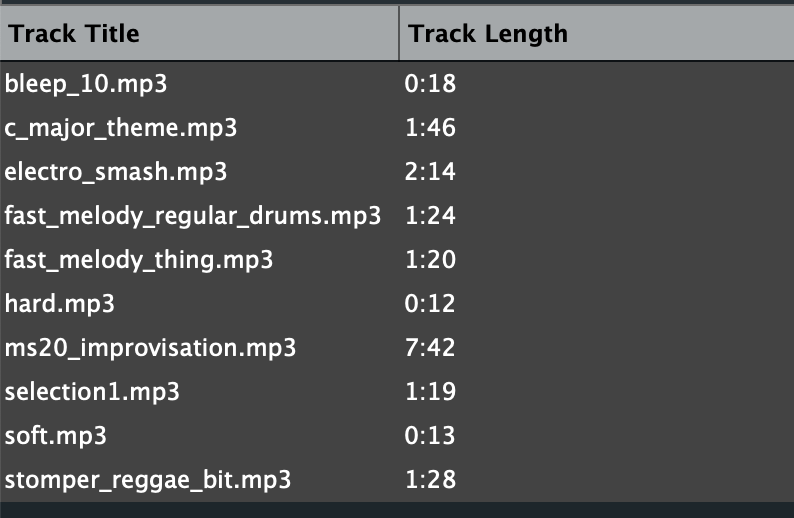
\includegraphics[width=8cm]{library.png}
	\caption{Library with tracks titles and lengths}
	\label{library}
\end{figure}

\subsection{R2C: Search}
Search functionality was implemented by adding a \texttt{Label} to enter text at the bottom of the player. Graphically, this was solved in the \texttt{PlaylistComponent} class with two labels, one for the title of the search box, and another for the search box itself. These are initialised in the constructor function as shown in \autoref{searchbox} and drawn with the usual \texttt{paint()} and \texttt{resize()} functions. A lambda function is attached to listen for changes to the search box contents.

\begin{listing}
	\begin{minted}{cpp}
	searchTitle.setText("Search (Hit Enter)", juce::dontSendNotification);
	searchTitle.attachToComponent(&searchInput, true);
	searchTitle.setJustificationType(juce::Justification::verticallyCentred);
	searchInput.setEditable(true);
	searchInput.setColour(juce::Label::backgroundColourId, juce::Colours::darkblue);

	// Lambda function to handle text inputs into the search box
	searchInput.onTextChange = [this] { searchLibraryFor(searchInput.getText()); };
	\end{minted}
	\caption{Initialising the search box}
	\label{searchbox}
\end{listing}

The actual search functionality is triggered in the \texttt{searchLibraryFor} function by traversing the vector of track titles and comparing the search term to those. JUCE provides a variety of classes to make this string search easier out of the box, as shown in \autoref{search}. The results are pushed to a new vector by flagging each vector position with a \texttt{true} or \texttt{false} value.

\begin{listing}
	\begin{minted}{cpp}
	void PlaylistComponent::searchLibraryFor(const String &searchTerm)
{
	searchResults.clear();

	// User needs to type at least two characters for the search to execute.
	// The search works by looking for a string in each element of the track titles vector.
	// We maintain a vector "searchResults" that is of equal length as track titles. If the track title matches our
	// search term, we mark our result vector as "true" in the same index position as the track title.
	// Later, we can check each track title against the results vector to decide how to show the user that a specific
	// track was a match (or not)
	if (searchTerm.length() > 1)
	{
		// Iterate over the track titles and look for the search term in each
		for (int i = 0; i < trackTitles.size(); ++i)
		{
			if (trackTitles[i].contains(searchTerm))
			{
				// Hit - mark this track as a result
				searchResults.push_back(true);
			}
			else
			{
				// Miss - mark this track as not a result
				searchResults.push_back(false);
			}
		}
	}
	\end{minted}
	\caption{Running a search}
	\label{search}
\end{listing}

This approach is used to highlight the results when drawing the library table. Each row's ID is compared to the results vector. If it is true, then the row is painted in a different color. The result is that matching search results are shown with a red background once the users hits enter after entering the search term, as shown in \autoref{searchfig}.

\begin{figure}[H]
	\centering
	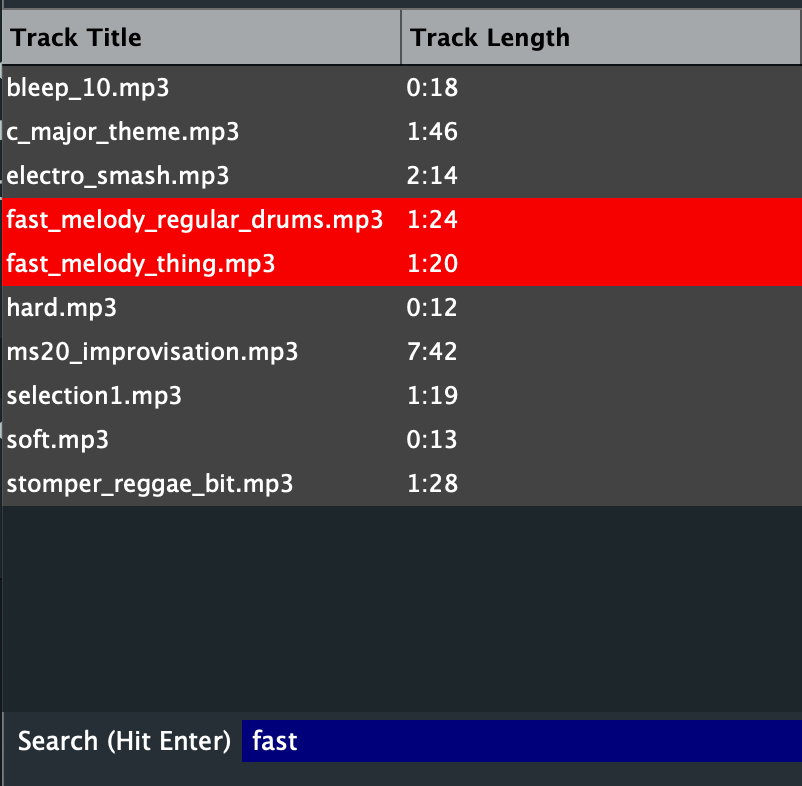
\includegraphics[width=6cm]{search.png}
	\caption{Search results highlighted}
	\label{searchfig}
\end{figure}

\subsection{R2D: Deck Playback}
The library was given a second column with additional buttons to address the left and right decks. In order to access the decks, the constructor of the library had to be extended to receive pointers to both decks, which are stored as private members of the \texttt{PlaylistComponent}. This allows us to then push a track to the respective deck on a button event as shown in \autoref{deckpush}. An additional \texttt{loadURL()} function was provided in the \texttt{DeckGUI} class, which in turn address the respective \texttt{loadURL()} interfaces of the \texttt{WaveformDisplay} and \texttt{DJAudioPlayer} classes. This retains proper abstraction from the music library to the underlying components of the deck. The left and right decks are addressed respectively by identifying the buttons with a component name of "Left" and "Right", respectively. This allows us to retain the component ID for both buttons on a single row, but still differentiate between the left and right button to know which deck to target.

\begin{listing}
	\begin{minted}{cpp}
void PlaylistComponent::buttonClicked(Button *button)
{
	// Convert the buttons component ID to an integer, so we can use it as the index of our track titles array
	int id = std::stoi(button->getComponentID().toStdString());

	// If the left button was clicked, push the track to the left deck
	if (button->getName() == "Left")
	{
		deck1->loadURL(URL{File{trackTitles[id]}});
	}

	// If the right button was clicked, push the track to the left deck
	if (button->getName() == "Right")
	{
		deck2->loadURL(URL{File{trackTitles[id]}});
	}
}
	\end{minted}
	\caption{Pushing tracks to the decks}
	\label{deckpush}
\end{listing}

The completed music library is shown in \autoref{endlibrary}.

\begin{figure}[H]
	\centering
	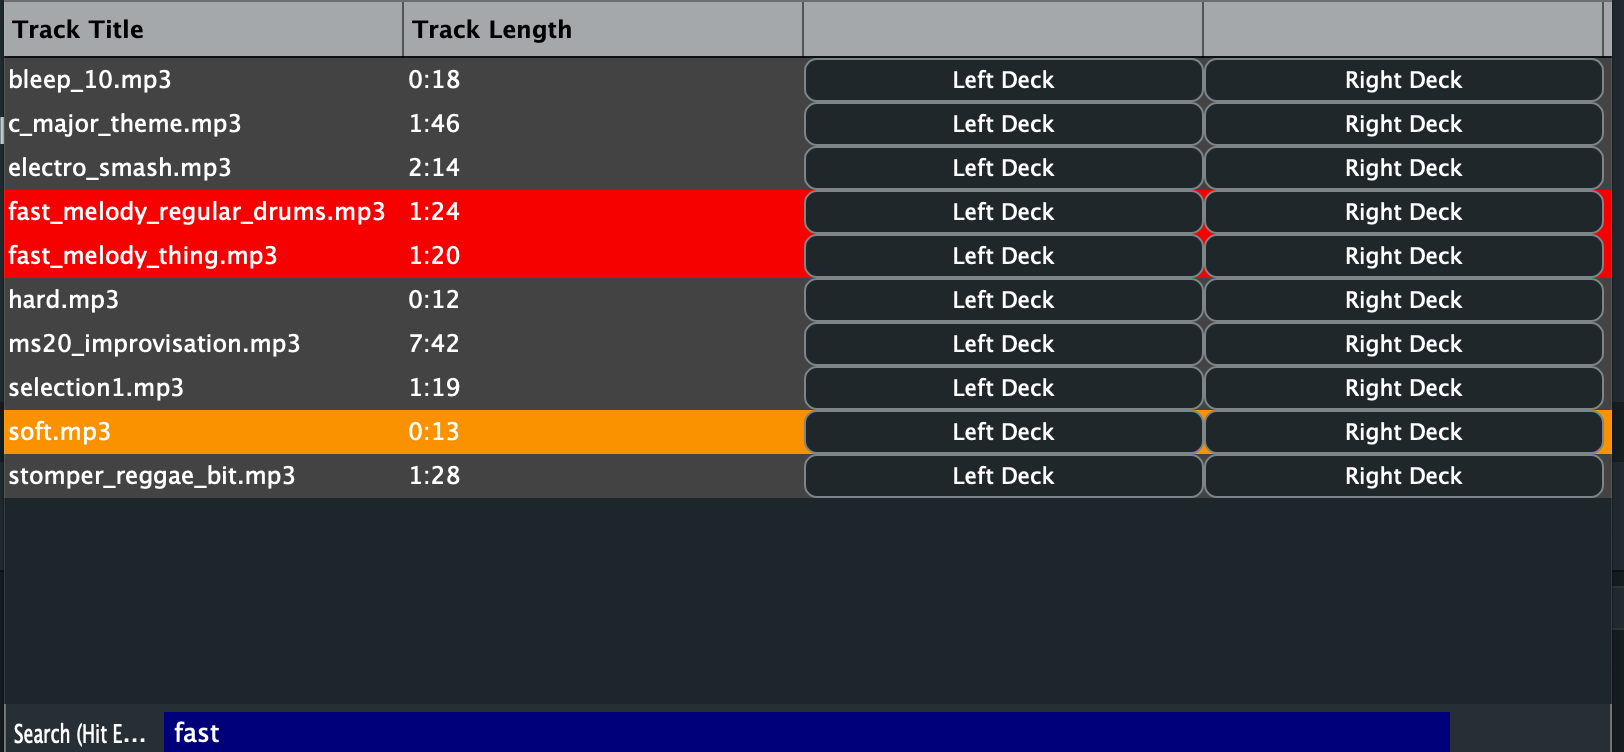
\includegraphics[width=12cm]{endlibrary.png}
	\caption{Finished music library}
	\label{endlibrary}
\end{figure}


\subsection{R2E: Library Persistence}
To achieve persistence of the library, the tracks are stored out to a text file as soon as they are dropped into the application. This is done by opening a \texttt{FileOutputStream} and streaming the vector of tracks to that text file. The file is stored in the user's music folder of the operating system. JUCE provides abstractions for addressing this folder in an OS-agnostic fashion.

Similarly, a \texttt{FileInputStream} is used in the constructor function of \texttt{PlaylistComponent} to read in the contents of a library file, if it already exists. JUCE provides functions to traverse a file line-by-line, and this was used to extract each line back into the track vector. Both reading and writing is shown in \autoref{IO}.

\begin{listing}
	\begin{minted}{cpp}
	/****** WRITING ******/
	// Store the music library to a text file on disk so we can retrieve it again
	// Create an output stream
	FileOutputStream libStream(library);
	// Write each loaded track to a new line in the library
	for (const String &trackTitle : trackTitles)
	{
		libStream << trackTitle << newLine;
	}

	/****** READING ******/

	if (library.existsAsFile())
	{
		FileInputStream libStream(library);
        trackTitles.clear();
        while (!libStream.isExhausted())
		{
			String currentTrack = libStream.readNextLine();
			trackTitles.push_back(currentTrack);
			trackLengths.push_back(getLengthOfTrack(currentTrack));
			tableComponent.updateContent();
		}
	}
	
	\end{minted}
	\caption{Reading and writing the music library}
	\label{IO}
\end{listing}


\section{Conclusion}

There is vast scope to build upon the application to add better UX, more functionality and more robust handling of files. This assignment was helpful in learning about object-oriented principles and the power of a highly object-oriented framework such as JUCE, which helps adopt these principles by enforcement.

\begin{thebibliography}{9}
	\bibitem{horton} 
	Horton, I., \& van Weert, P. (2018). \emph{Beginning C++17: From Novice to Professional}. Berkeley, CA: Apress.
	
	\bibitem{juce}
	Raw Material Software Limited, \emph{JUCE Class Reference List}. Retrieved 19 September 2020 from \url{https://docs.juce.com/master/index.html}.
	
\end{thebibliography}

\end{document}